\documentclass{beamer}
\setbeamertemplate{caption}[numbered]

\usetheme{Madrid}

% locale settings 
\usepackage[T2A]{fontenc}
\usepackage[utf8]{inputenc}
\usepackage[english,russian]{babel}

% graphics settings
\usepackage[compatibility=false]{caption}
\usepackage{subcaption}
\usepackage{wrapfig}
\usepackage{graphics, graphicx}
\graphicspath{{./images/}}

% hyperlinks settings
\usepackage{hyperref}
\hypersetup{unicode=true}

\title{Анализ данных кинопоиска}
\author[ПриМат]{Курносов Дмитрий, Лансков Никита,Нахатович Михаил, Смольский Максим}
\institute[Политех]
{
	Институт прикладной математики и механики, СПБПУ
}
\date{18 декабря, 2020}

\begin{document}
	\frame {
		\titlepage
	}
	\frame {
		\frametitle{Кратко о кинопоиске}
		
		КиноПоиск - крупнейший русскоязычный интернет-сервис о кино. Содержит
		информацию о различных фильмах, которой мы воспользовались для решения 
		поставленных статистических и исследовательских задач.
	}
	\frame {
		\frametitle{Архитектура проекта}
		\begin{figure}
			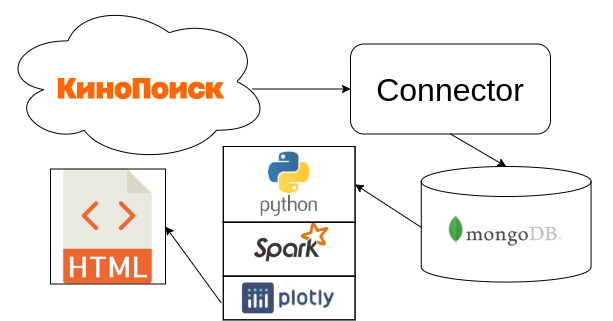
\includegraphics[width=\linewidth]{architecture}
		\end{figure}
	}
	\frame {
		\frametitle{Получение данных}
		\begin{figure}
			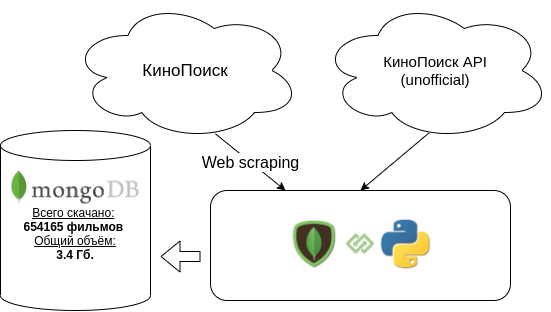
\includegraphics[width=\linewidth]{gettingData}
		\end{figure}
	}	
	\frame {
		\frametitle{Структура данных}
		\begin{figure}
			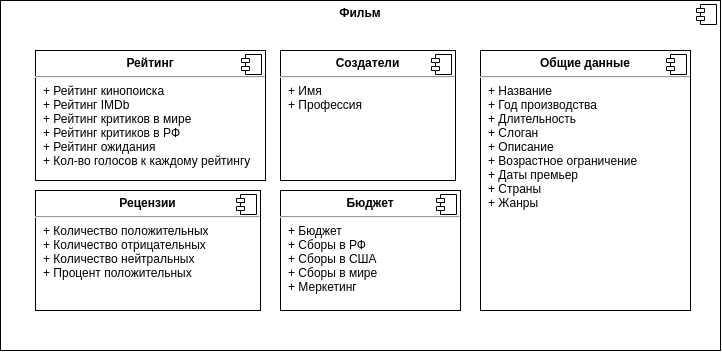
\includegraphics[width=\linewidth]{dataStructure}
		\end{figure}
	}
	\frame {
		\frametitle{Статистические задачи}

		\begin{itemize}
			\item \textbf{Корелляция оценок зрителей и критиков}
			\item Корелляция рейтинга КиноПоиска и рейтинга IMDb
			\item \textbf{Распределение фильмов по странам}
			\item \textbf{Распределение фильмов по прибыльности}
			\item \textbf{Распределение фильмов между странами по годам}
			\item \textbf{Распределение фильмов по возрастным ограничениям и годам}
			\item \textbf{Средний рейтинг российских фильмов по годам}
		\end{itemize}
	}
	\frame {
		\frametitle{Корелляция оценок зрителей и критиков}
		\begin{figure}
 			\centering
			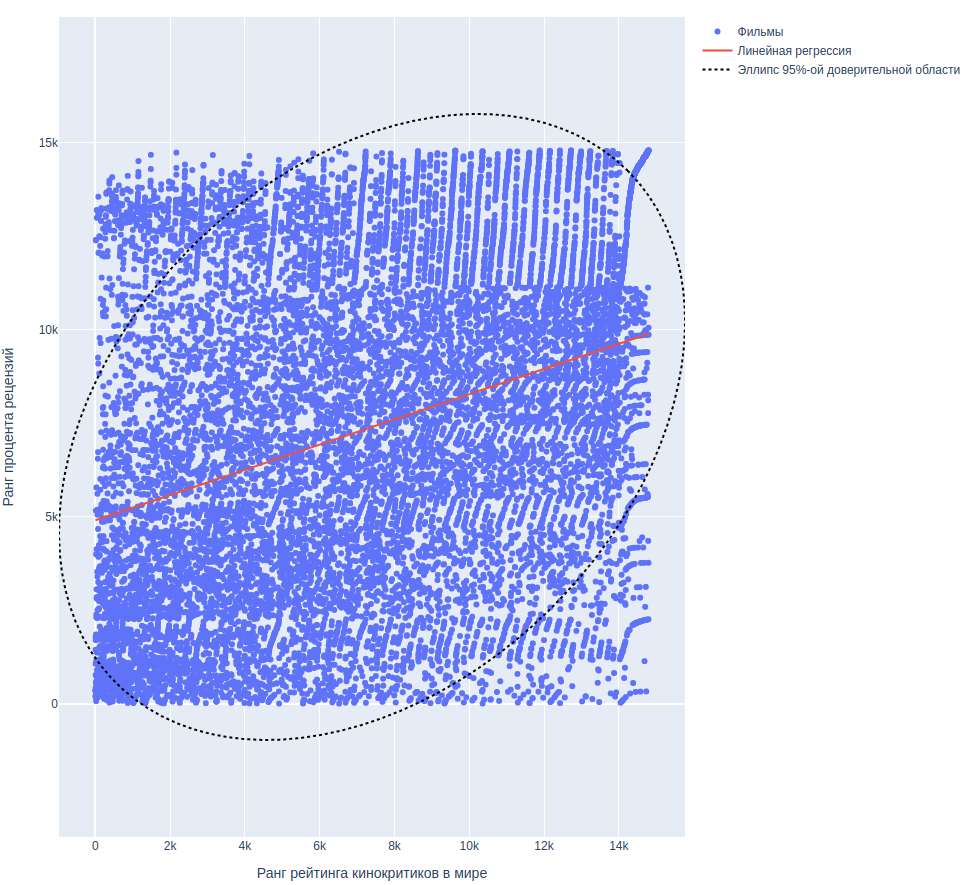
\includegraphics[width=0.6\linewidth]{corr/spirmen}
		\end{figure}
	}
	\frame {
		\frametitle{Корелляция рейтинга КиноПоиска и рейтинга IMDb}
	}
	\frame {
		\frametitle{Распределение фильмов по странам}
		\begin{figure}
 			\centering
			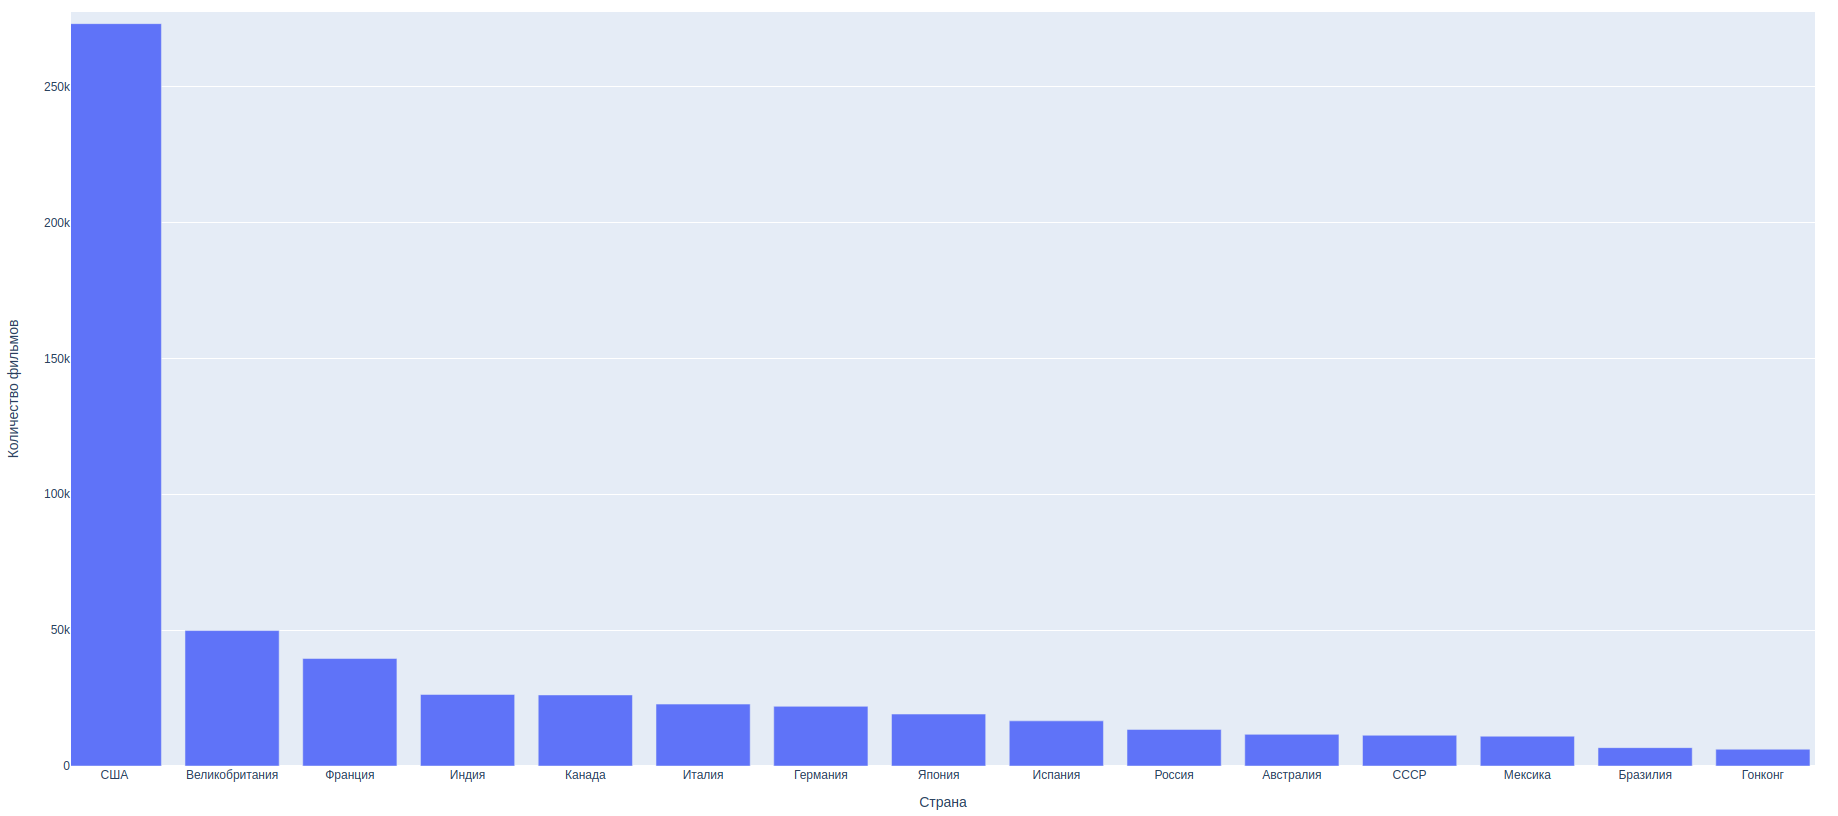
\includegraphics[width=\linewidth]{films_by_country/2}
		\end{figure}
	}
	\frame {
		\frametitle{Распределение фильмов по прибыльности (1/3)}
		\begin{figure}
			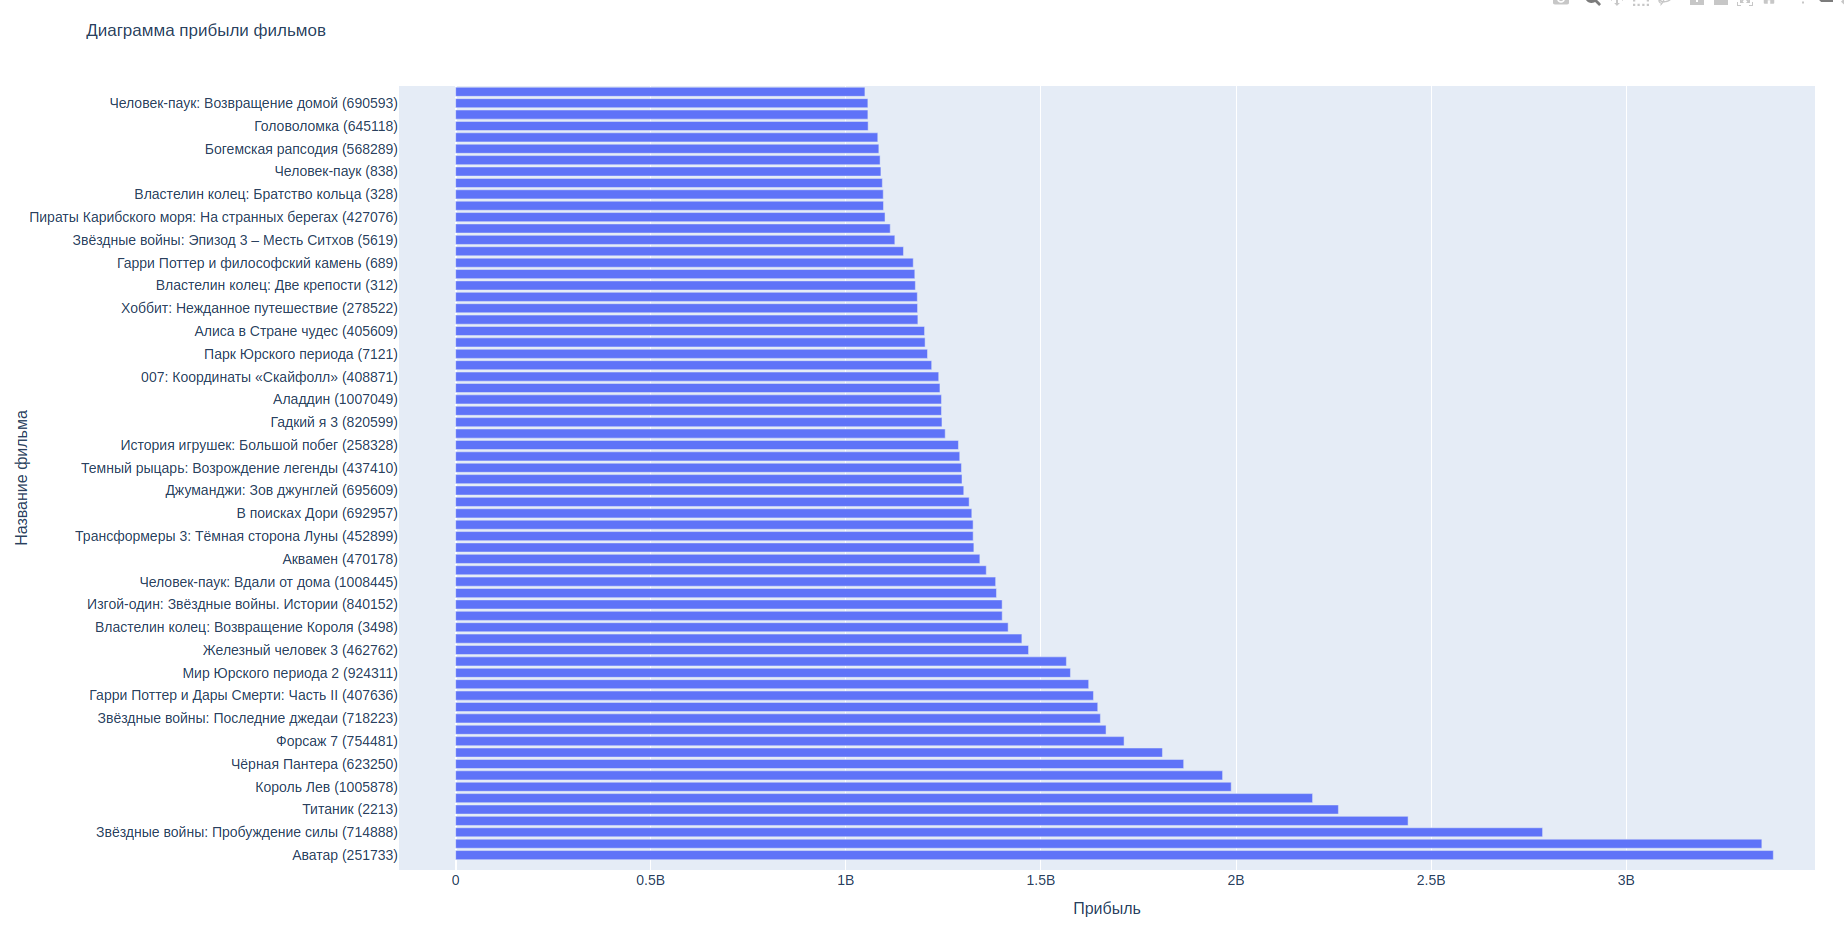
\includegraphics[width=\linewidth]{profit/best}
		\end{figure}
	}
	\frame {
		\frametitle{Распределение фильмов по прибыльности (2/3)}
		\begin{figure}
			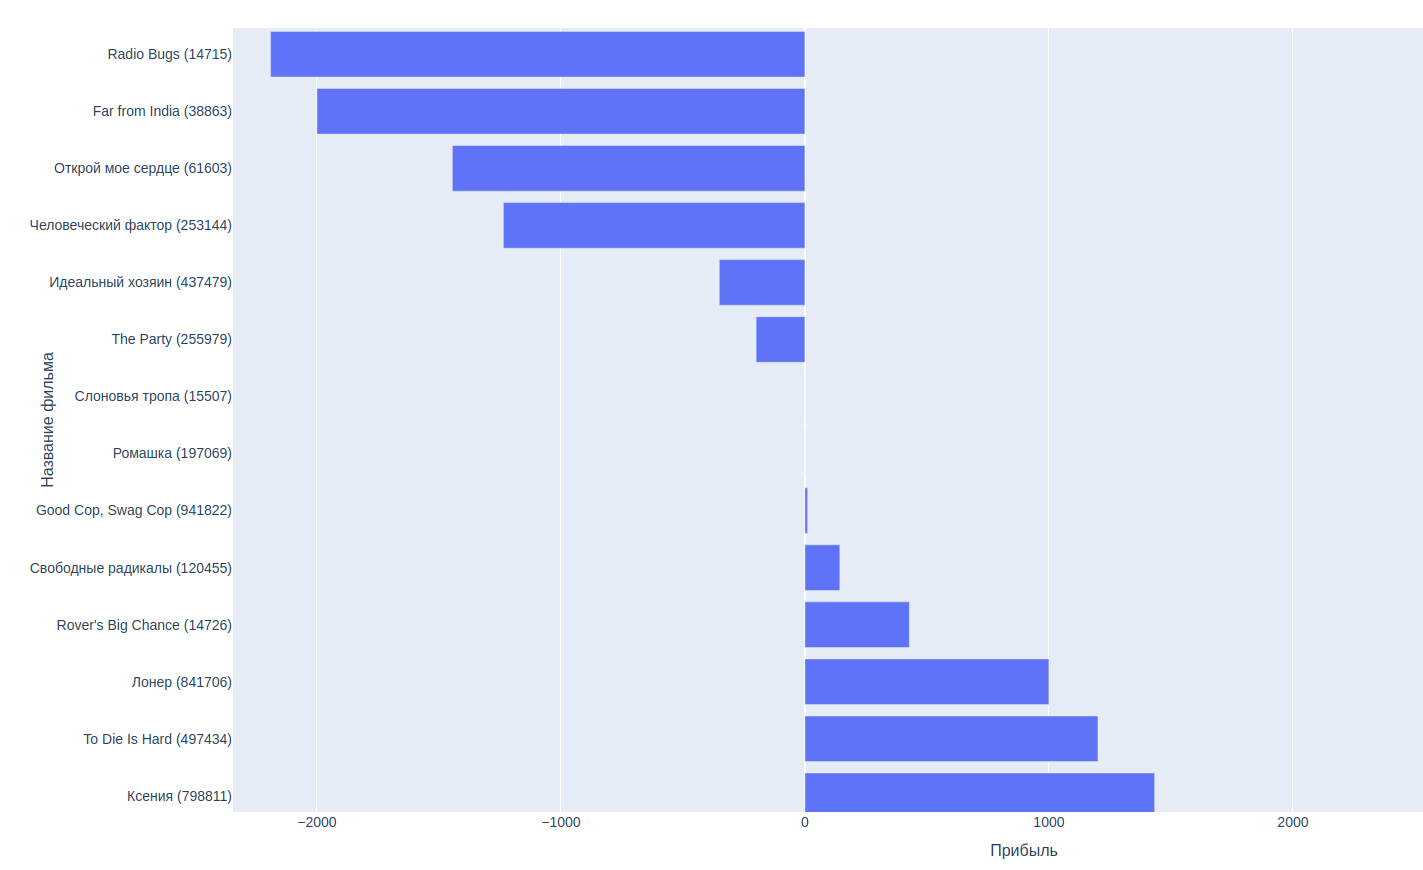
\includegraphics[width=\linewidth]{profit/zero}
		\end{figure}
	}
	\frame {
		\frametitle{Распределение фильмов по прибыльности (3/3)}
		\begin{figure}
			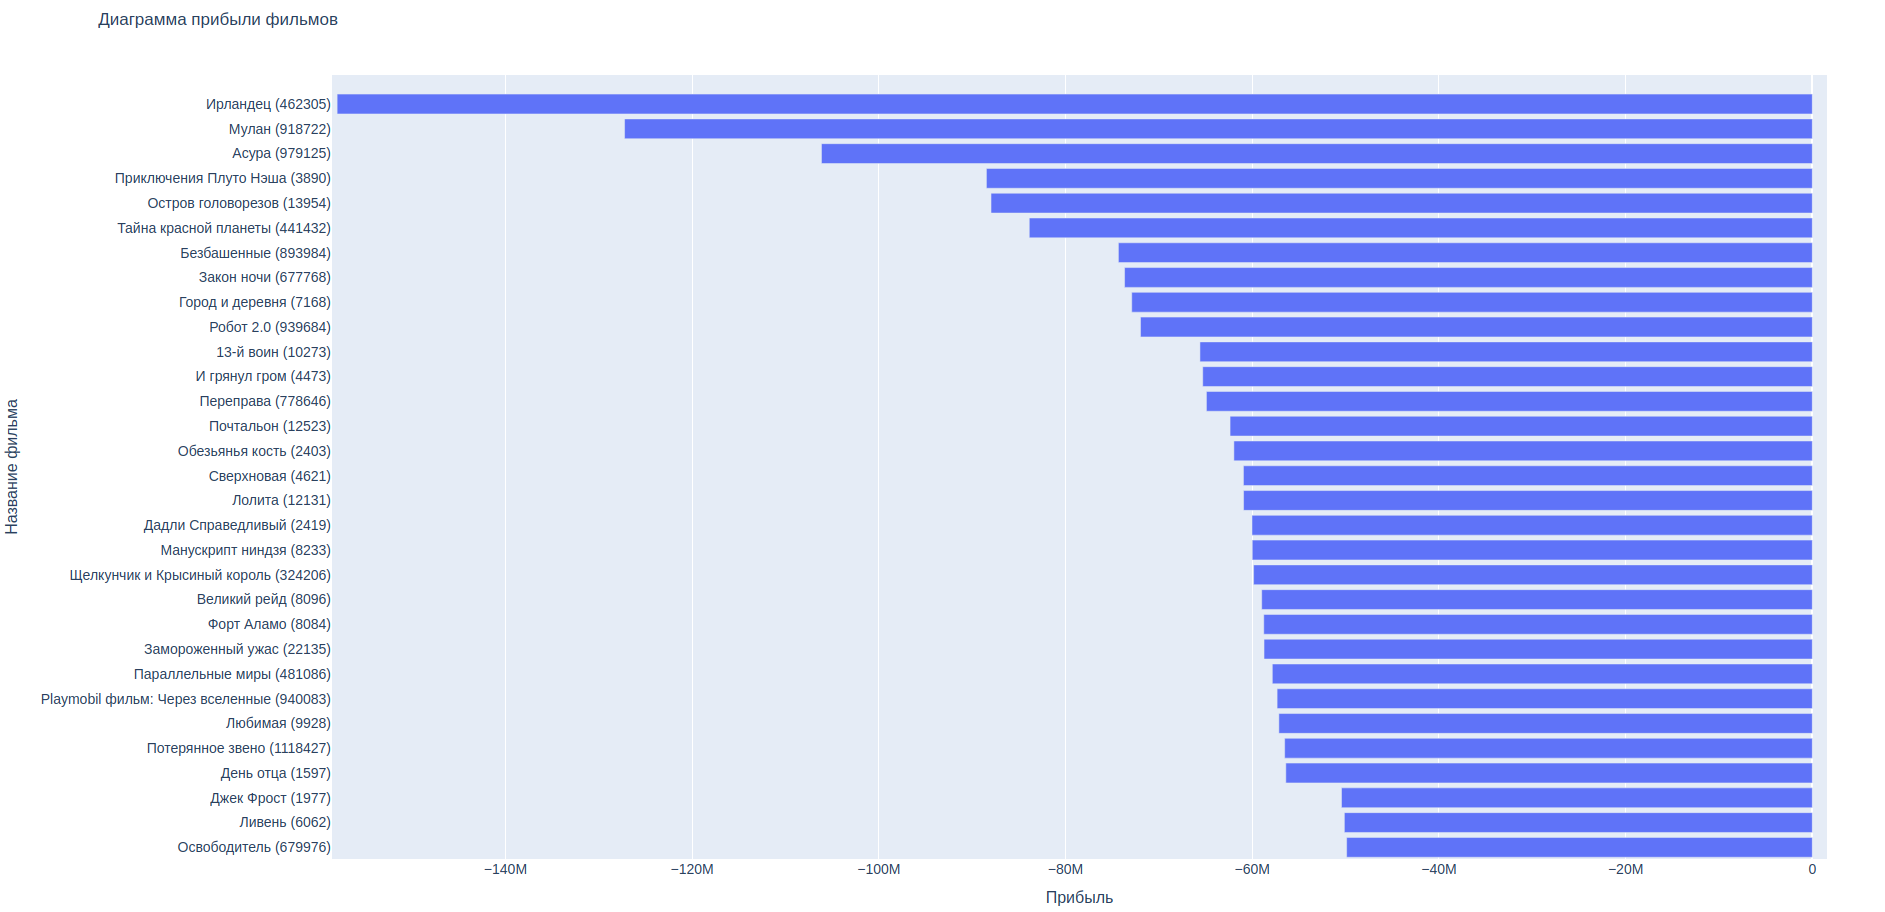
\includegraphics[width=\linewidth]{profit/worst}
		\end{figure}
	}
	\frame {
		\frametitle{Распределение фильмов между странами по годам (1/2)}
		\begin{figure}
			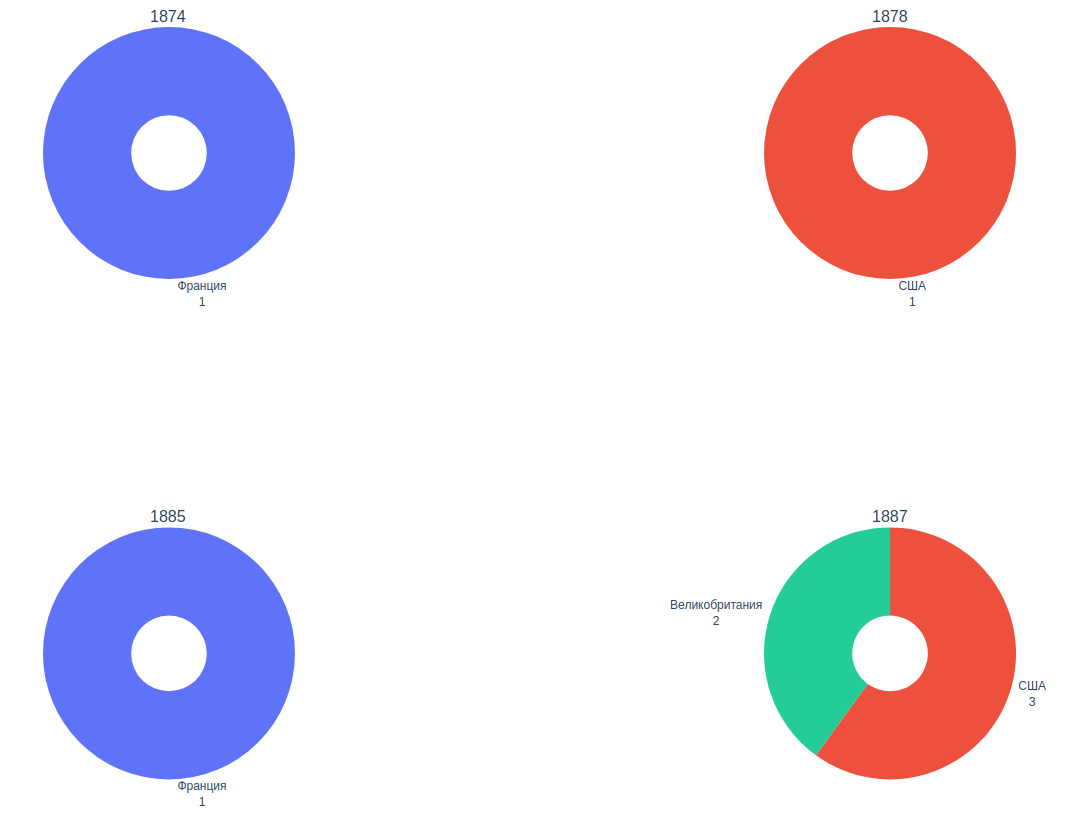
\includegraphics[width=0.8\linewidth]{films_countries_year/1}
		\end{figure}
	}
	\frame {
		\frametitle{Распределение фильмов между странами по годам (2/2)}
		\begin{figure}
			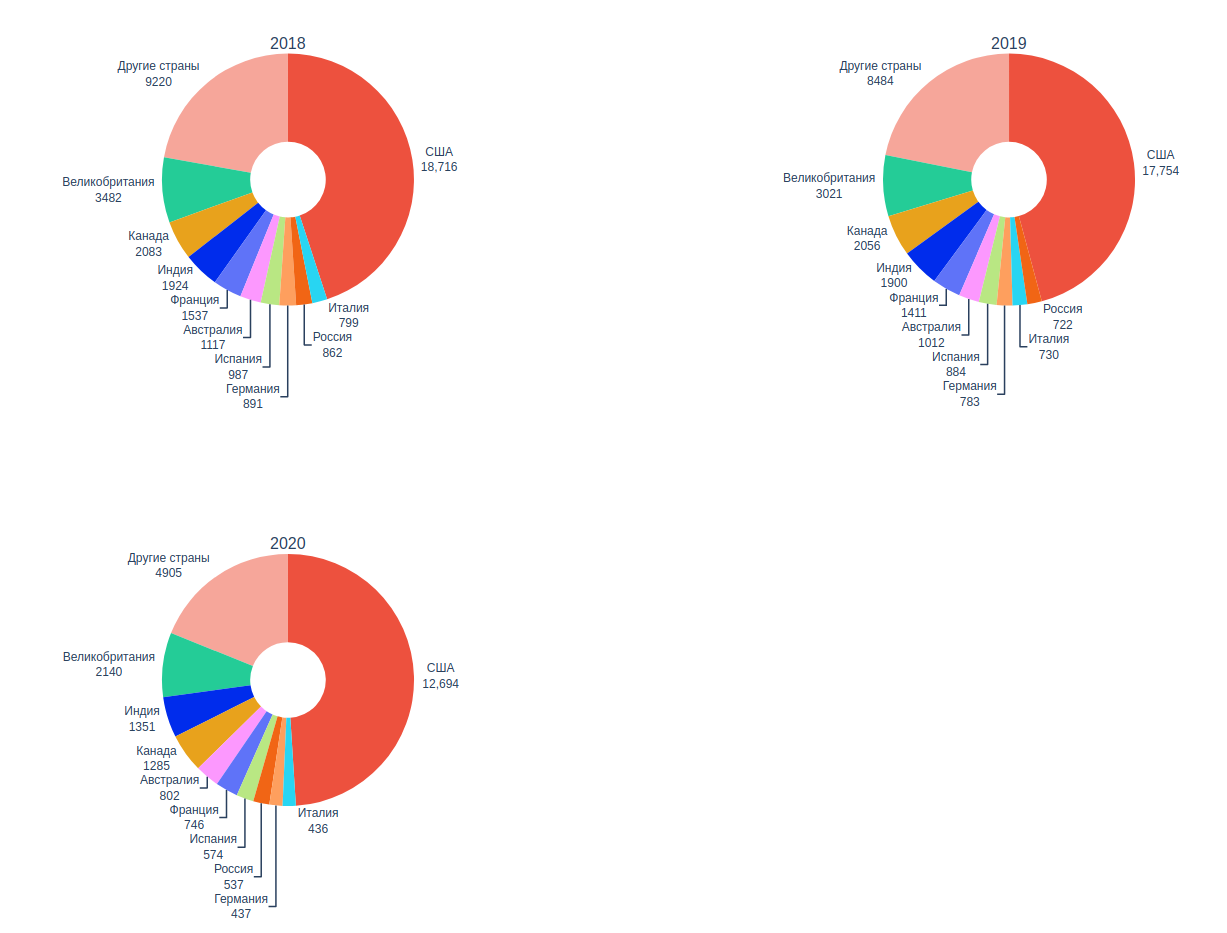
\includegraphics[width=0.8\linewidth]{films_countries_year/2}
		\end{figure}
	}
	\frame {
		\frametitle{Распределение фильмов по возрастным ограничениям и годам}
		\begin{figure}
			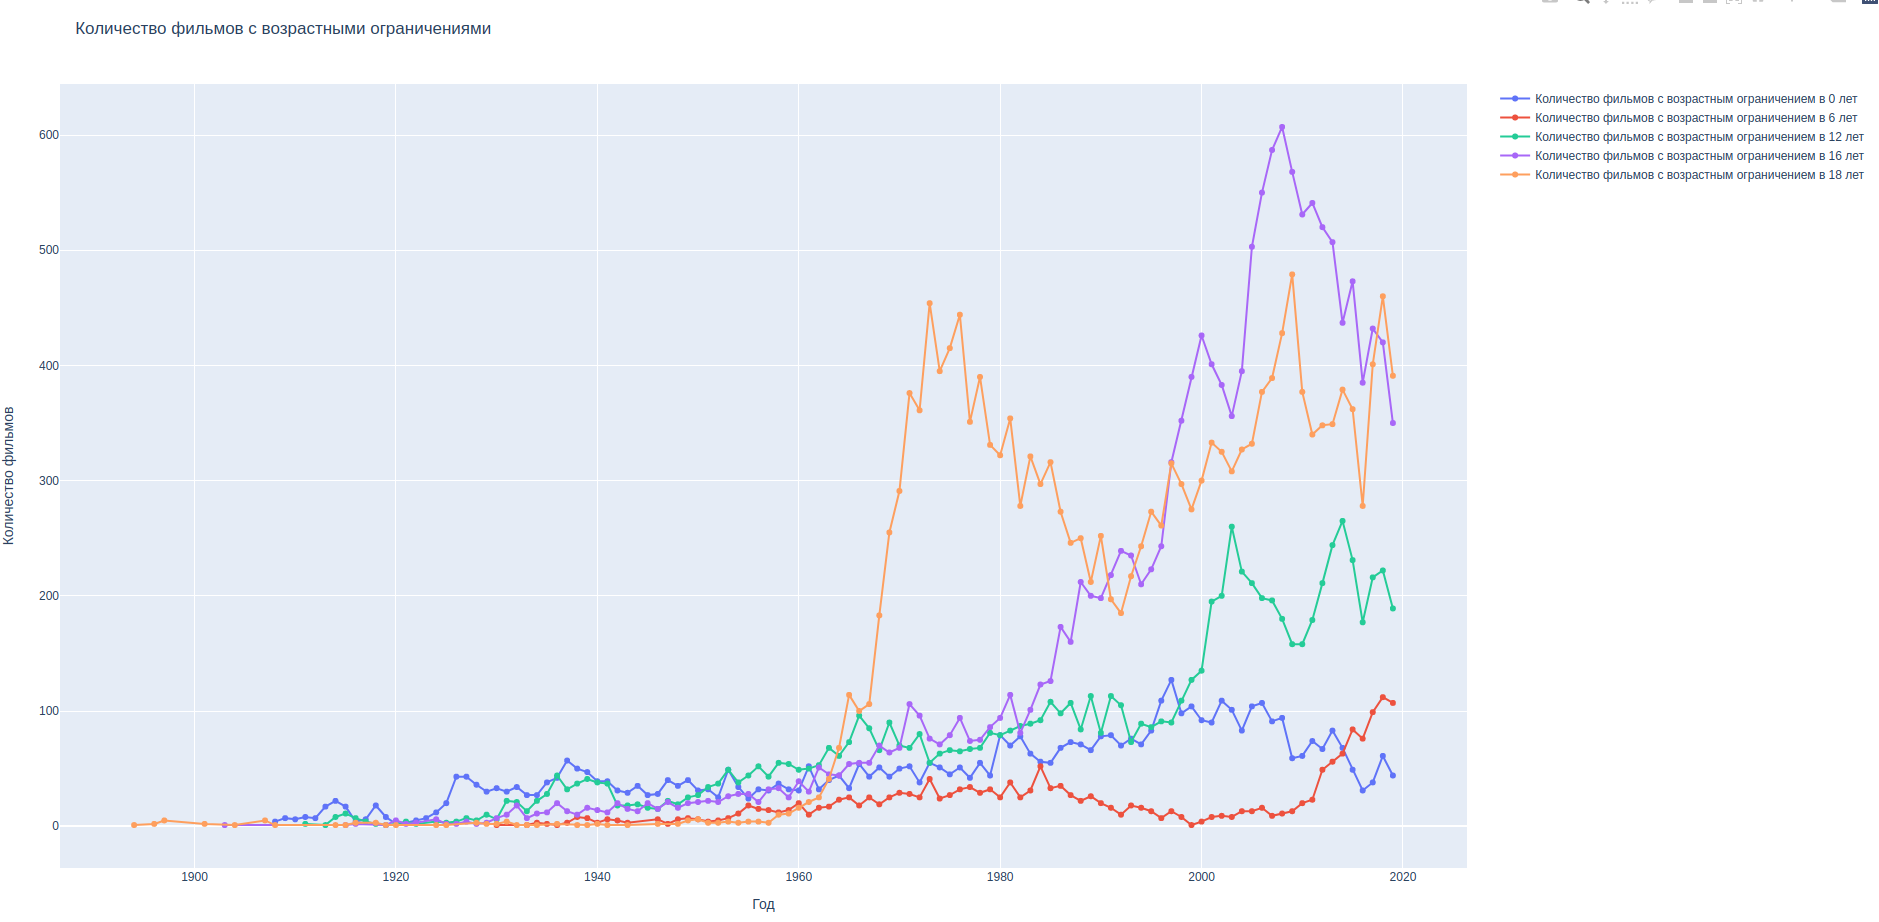
\includegraphics[width=\linewidth]{years_restrict/1}
		\end{figure}
	}	
	\frame {
		\frametitle{Средний рейтинг российских фильмов по годам}
		\begin{figure}
			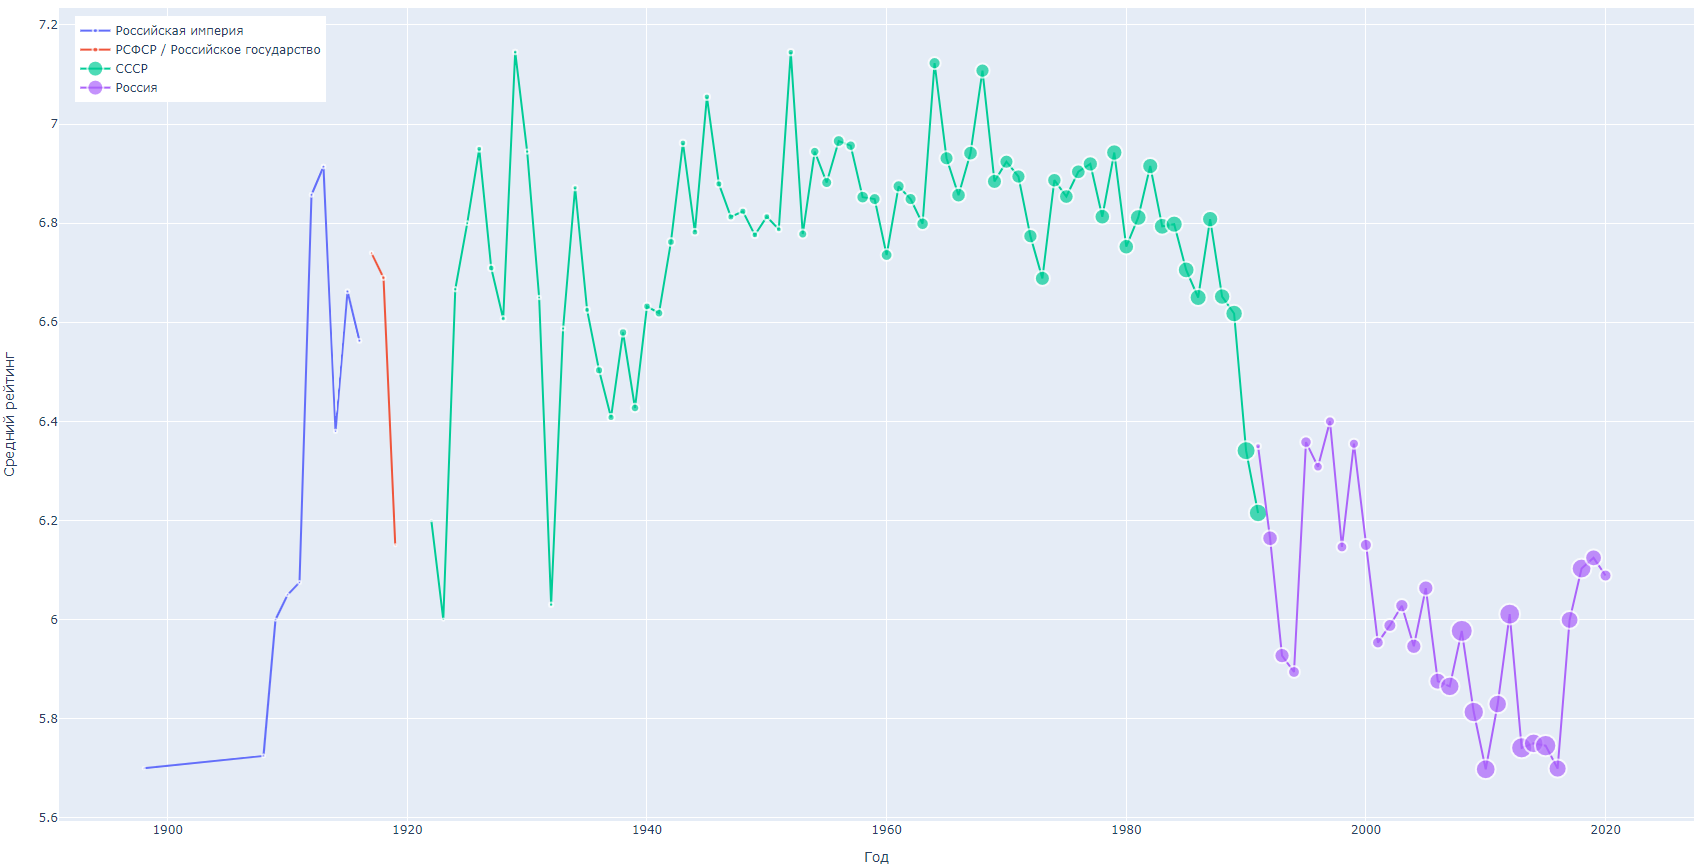
\includegraphics[width=\linewidth]{russia_rating/1}
		\end{figure}
	}	

	\frame {
		\frametitle{Исследовательские задачи}
		
		\begin{itemize}
			\item Прогноз количества фильмов по жанрам на 10 лет
		\end{itemize}
	}
	\frame {
		\frametitle{Прогноз количества фильмов по жанрам на 10 лет (1/4)}
		\begin{figure}
			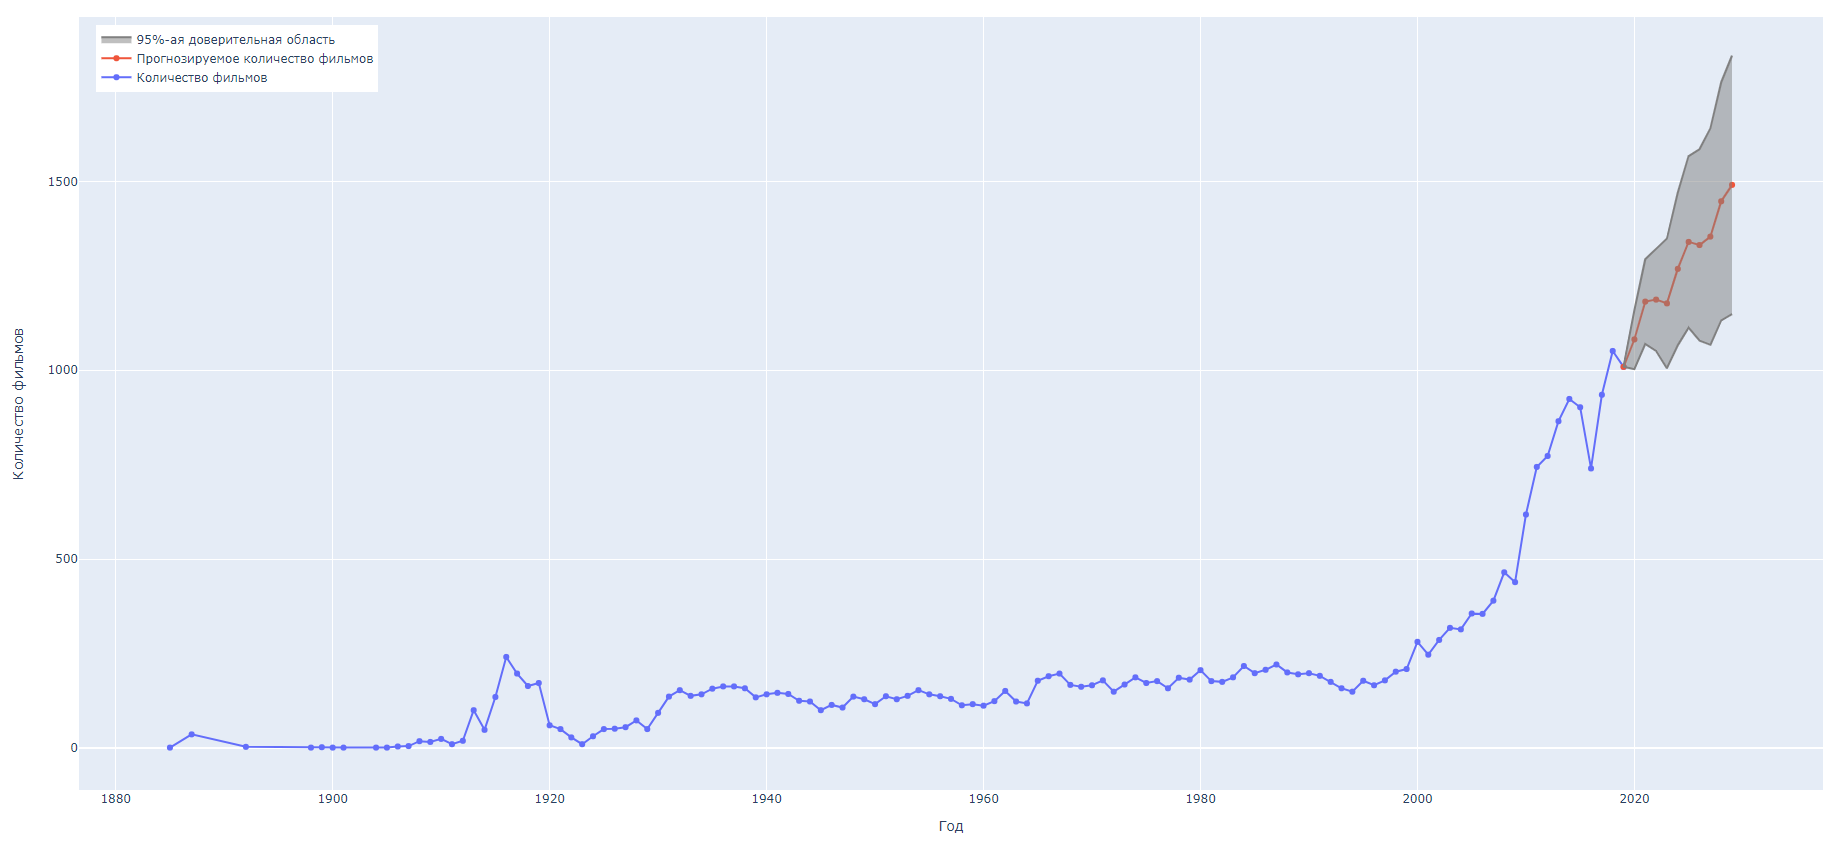
\includegraphics[width=\linewidth]{genre_predict/cartoons}
		\end{figure}
	}	
	\frame {
		\frametitle{Прогноз количества фильмов по жанрам на 10 лет (2/4)}
		\begin{figure}
			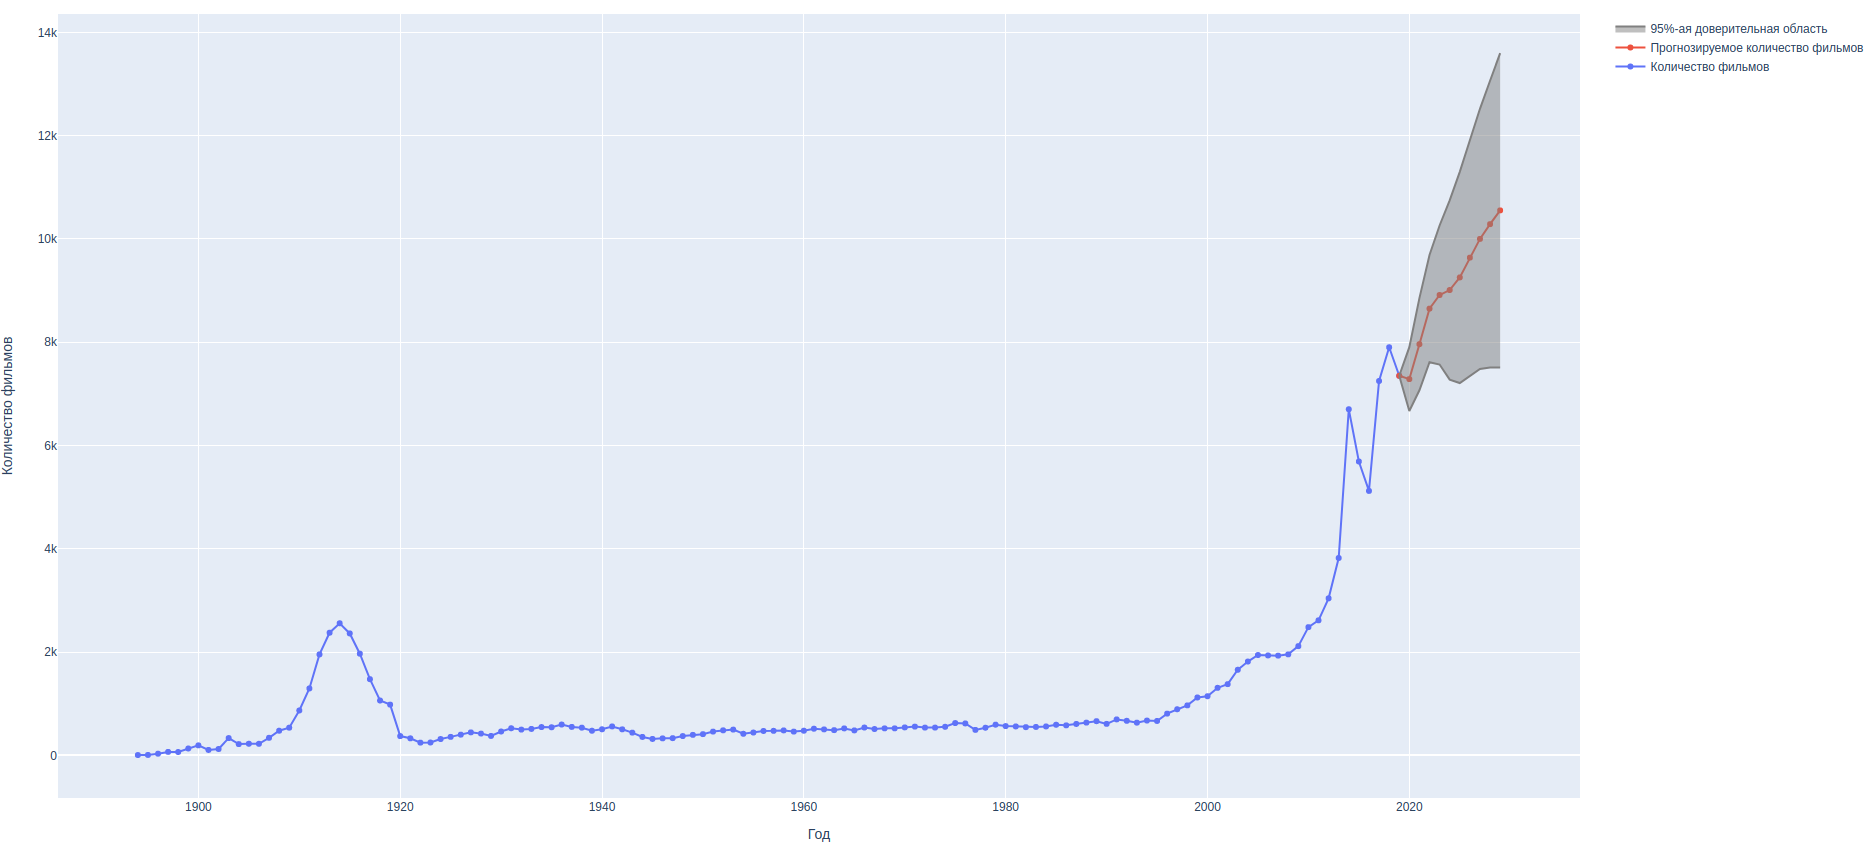
\includegraphics[width=\linewidth]{genre_predict/comedy}
		\end{figure}
	}	
	\frame {
		\frametitle{Прогноз количества фильмов по жанрам на 10 лет (3/4)}
		\begin{figure}
			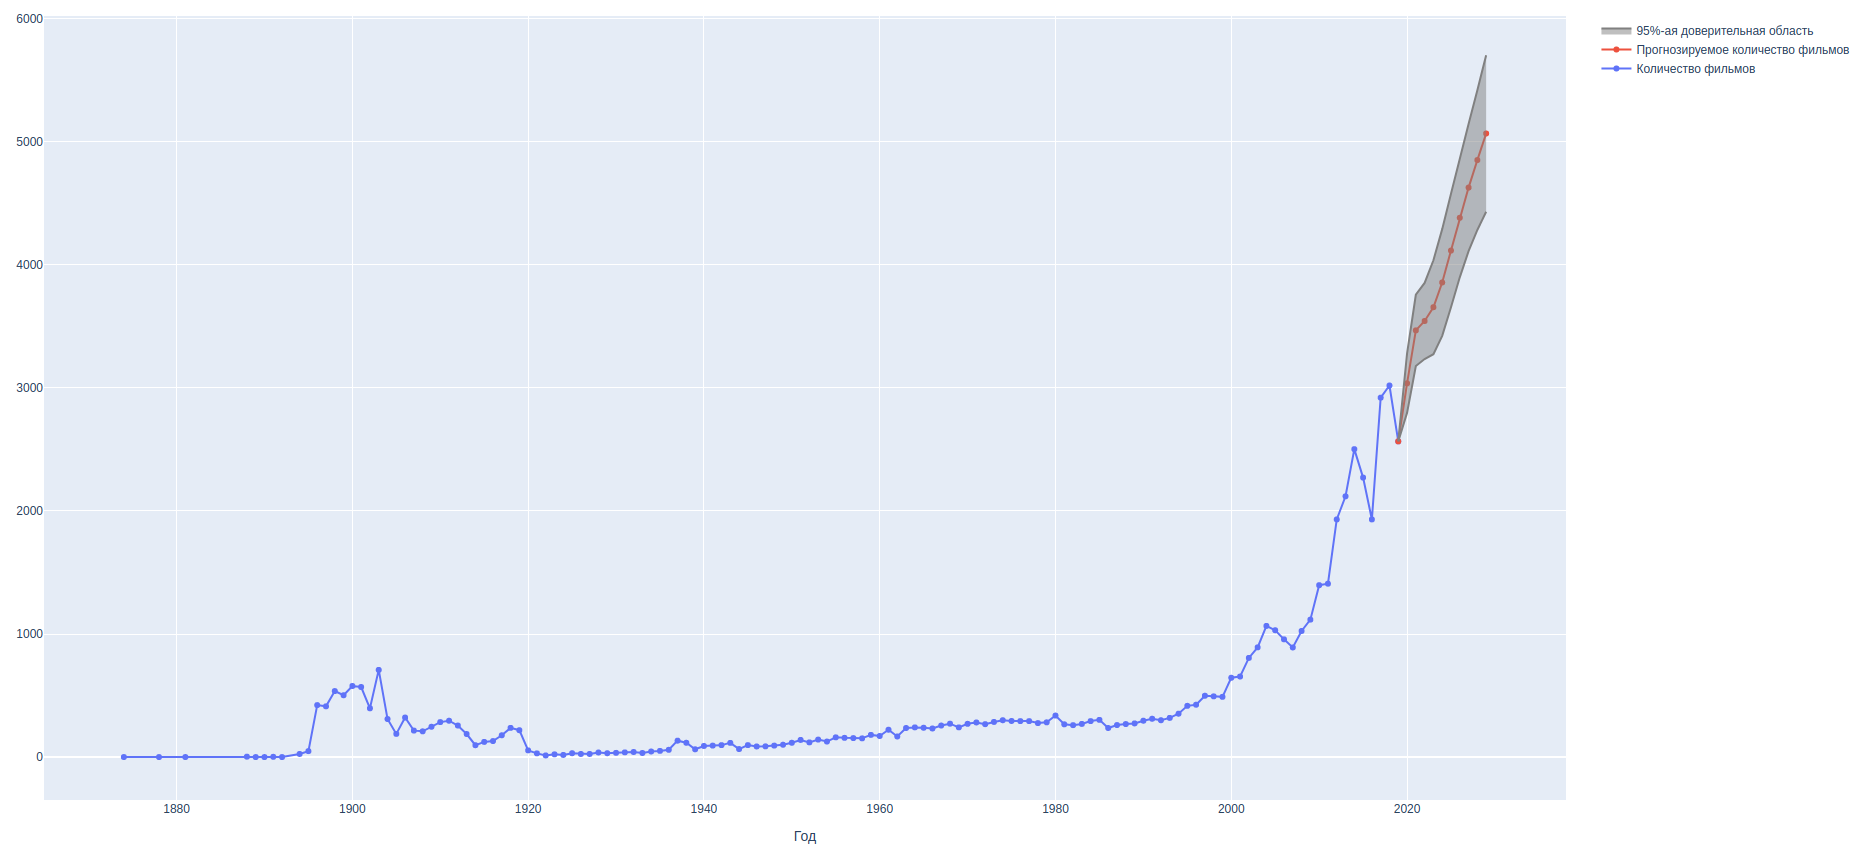
\includegraphics[width=\linewidth]{genre_predict/documental}
		\end{figure}
	}	
	\frame {
		\frametitle{Прогноз количества фильмов по жанрам на 10 лет (4/4)}
		\begin{figure}
			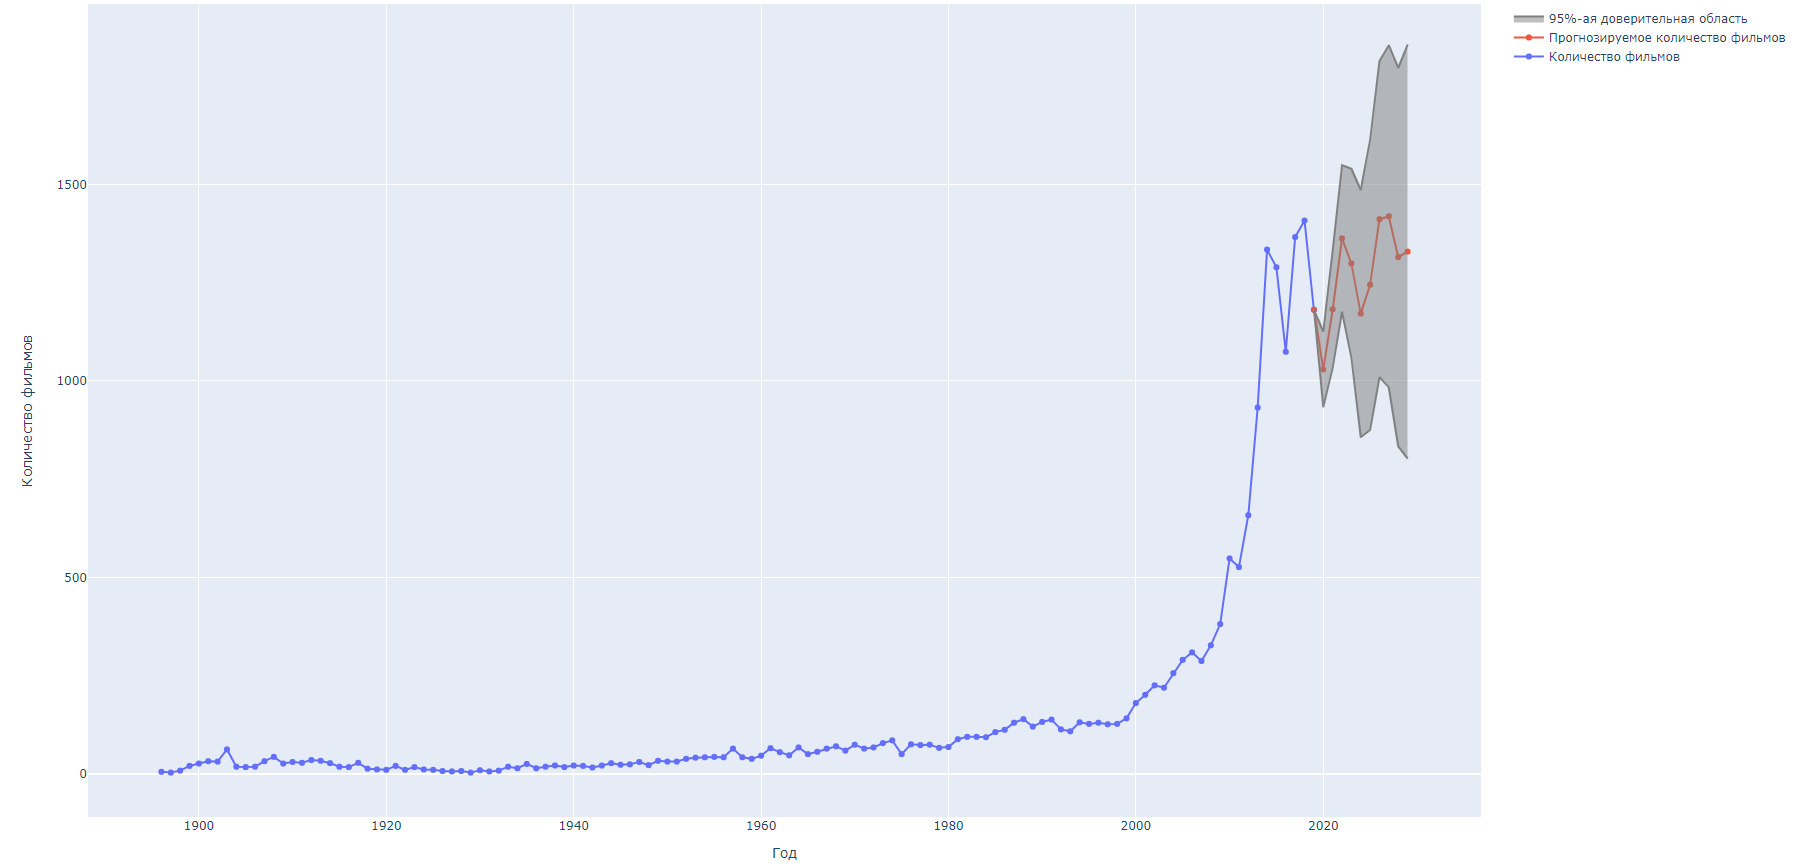
\includegraphics[width=\linewidth]{genre_predict/fantasy}
		\end{figure}
	}	
	\frame {
		\frametitle{Дальнейшие исследования}
		
		\begin{itemize}
			\item Предсказание рейтинга фильма по его создателям и другим данным
			\item Включить в рассмотрение сериалы
			\item ...
		\end{itemize}
	}

\end{document}